
\documentclass{tufte-handout}

\usepackage{amsmath}
\usepackage{graphicx}

\title{Multiple Partition Regression Analysis}
\author{Rhys Hawkins and Malcolm Sambridge}

\usepackage{units}

\usepackage{fancyvrb}
\fvset{fontsize=\tiny}

\usepackage{listings}
\lstset{basicstyle=\tiny, numbers=left, frame=single, language=Python}

\begin{document}

\maketitle

\begin{abstract}

This tutorial describes how to analyse discontinuous data using Monte-Carlo
Markov-Chain based regression.

\end{abstract}

\section{Pre-requisites}

This tutorial is for the Python version of the rjmcmc library. The examples
rely on the Matplotlib library for plotting. The versions used in the 
development of this tutorial are as follows:

\begin{itemize}
\item Python 2.7.1
\item rjmcmc 0.1.0
\item Matplotlib 1.1.0
\end{itemize}

\section{The Data}

Similar to the single partition tutorial we will use a non-trivial 
synthetic dataset with added noise. The difference this time is that 
we will add a series of discontinuities or step functions and a sign
change.

The base function that is used is an exponentially increasing sine wave over 
the domain 0 $\ldots$ 10, ie:

\begin{equation}
y = \mathrm{stepsign}(x) \times e^\frac{x}{3} \sin{ \frac{2x}{3}} + \mathrm{step}(x)
\end{equation}

Where the $\mathrm{step}$ and $\mathrm{stepsign}$ functions are
defined as follows:

\begin{equation}
\mathrm{step}(x) = \left\{ \begin{array}{rl}
15 & x < 2.5 \\
-20 & 2.5 \ge x < 5 \\
0 & {\mathrm otherwise} \\
\end{array}
\right.
\end{equation}

\begin{equation}
\mathrm{stepsign}(x) = \left\{ \begin{array}{rl}
-1 & x < 2.5 \\
1 & 2.5 \ge x < 5 \\
-1 & {\mathrm otherwise} \\
\end{array}
\right.
\end{equation}

\begin{marginfigure}
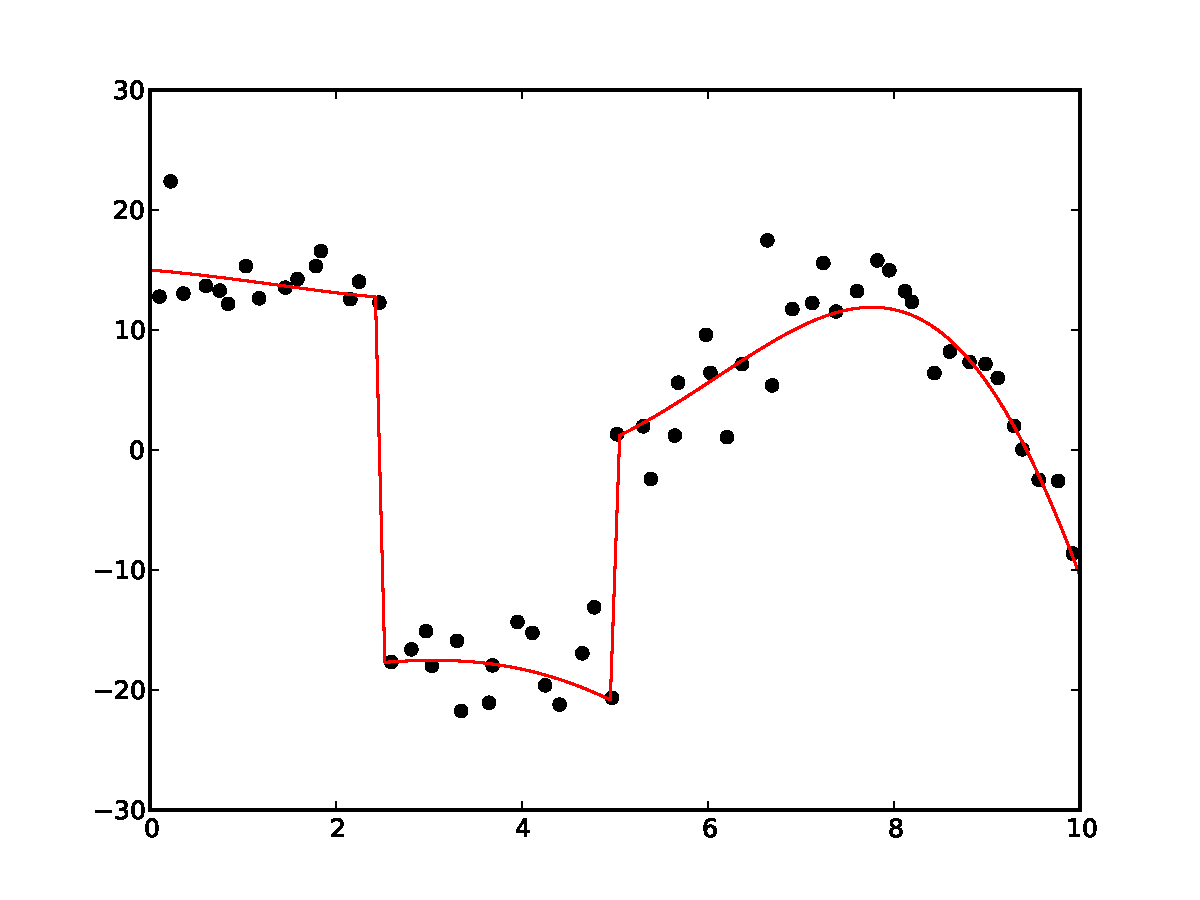
\includegraphics[width=\linewidth]{../ch0-exampledata.pdf}
\caption{The Synthetic Data}
\label{fig:syntheticdata}
\end{marginfigure}

The actual dataset unevenly (though with fairly good coverage) samples
this function and adds some Gaussian noise and these values are save
to an ASCII text file. A plot of the synthetic data points with the 
true function is shown in Figure~\ref{fig:syntheticdata}.

\section{Loading the Data}

For those unfamiliar with Python, we discuss briefly the loading of data
from a simple ASCII text file. The code for loading the data and doing
a simple plot is shown in Listing~\ref{lst:loadingdata}.

\lstset{caption=Loading the Data,label=lst:loadingdata}
\lstinputlisting{../ch1-loading.py}

The ASCII file contains an x, y pair per line separated by a space. On
line 12, we use the built in function {\tt open} to open the file. One
lines 15 and 16 we initialize 2 list that will contain the x and y 
coordinates in the file. On line 18 we loop through the lines in the 
file and add each x, y pair to the 2 separate lists.

\begin{marginfigure}
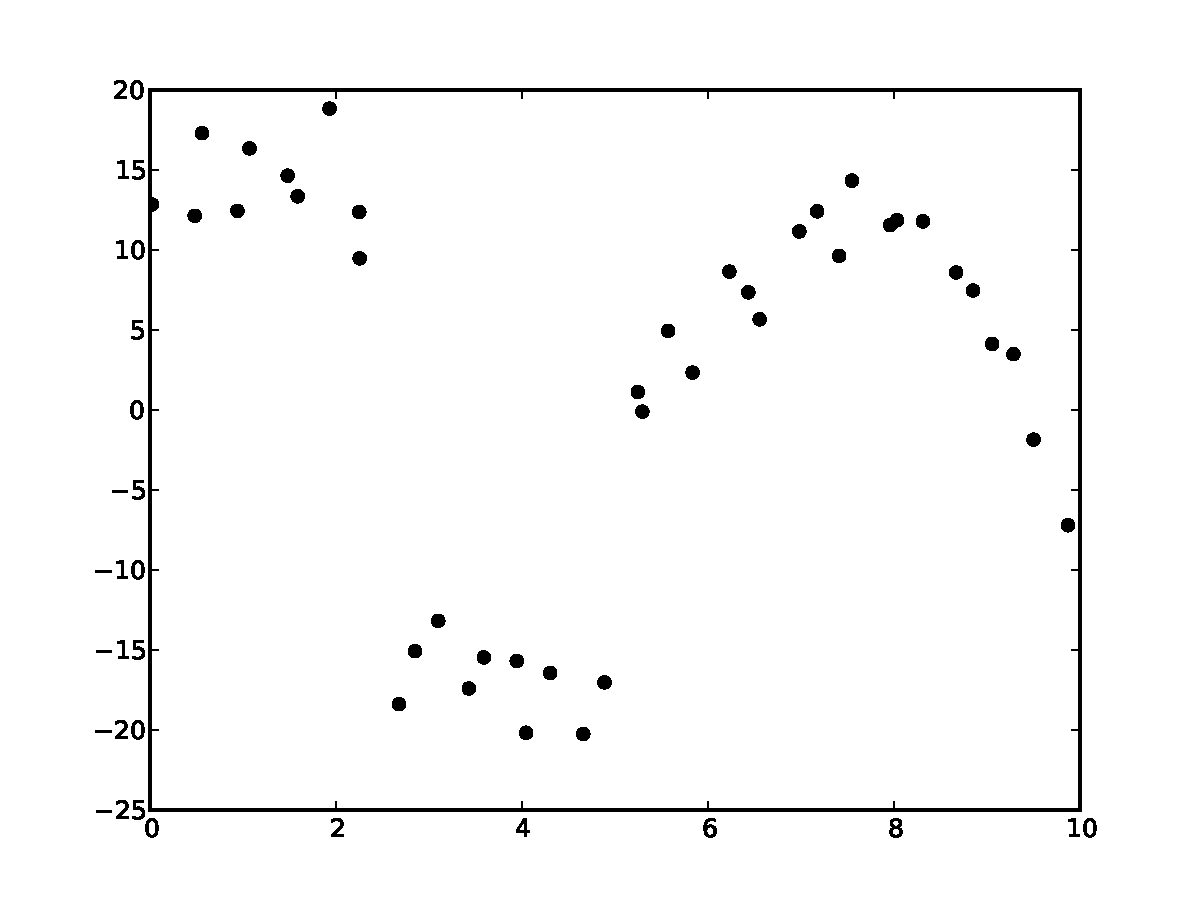
\includegraphics[width=\linewidth]{../ch1-loading.pdf}
\caption{The Plot of the Data}
\label{fig:loading}
\end{marginfigure}

From line 26 onwards, we plot the data using the matplotlib library
and save the plot to a PDF file. The plot resulting from this script
can be seen in Figure~\ref{fig:loading}.

\section{Running the default analysis}

For performing a regression analysis on a continuous dataset the
function is called {\tt regression\_part1d}. The parameters for this
function are mostly the same as the {\tt regression\_single1d}
function with the only additional required parameter being {\tt pd}.

The complete list of parameters for this function are as follows with
default values shown where applicable:

\begin{description}
\item[dataset] The dataset object to run the analysis on. This is an
  rjmcmc.dataset1d object which wraps the x and y vectors you load
  from the file and includes individual point noise values. This is
  the only parameter which doesn't have a default value.
\item[pd] The standard deviation for the perturbation of partition
  boundaries.
\item[burnin = 10000] The number of initial samples to throw away.
\item[total = 50000] The total number of samples to use for the
  analysis.
\item[max\_order = 1] The maximum order of polynomial to use to fit
  the data.
\item[xsamples = 100] The number of points to sample along the x
  direction for the curve.
\item[ysamples = 100] The number of points to sample along the y
  directory for the statistics such as mode, median and confidence
  intervals. This is the number of bins for the histograms in the y
  direction.
\item[confidence\_interval = 0.95] The confidence interval to use for
  minimum and maximum confidence intervals. This should be a value
  between 0 and 1.
\end{description}

For this analysis we are only going to use the default values and the
listing is shown in Listing~\ref{lst:defaultanalysis}.

\lstset{caption=Running the Default Analysis,label=lst:defaultanalysis}
\lstinputlisting{../ch2-analyse.py}

The preamble (lines 1 $\ldots$ 24) consists of loading the file as in
the previous section.

An important part of the analysis is estimating the error in the data.
This is specified as a error value per data point and can be thought
of a weighting as to how well the fit will attempt to fit an
individual point. If the value is low, then the fit will be tight and
conversely if the value is high then the fit will be loose. On lines
35 and 36 we set a value of 3.0 for all data points.  Use this value
for now, but try other values greater than 0.0 to see the effect.

On line 41 we construct the dataset1d object from the x, y and n lists
we created.  These lists must be the same length.

On line 46 we set the value for the pd parameter. With partition
modelling, a variable number of discontinuities are trialed at random
locations along the x-axis. As part of the fitting process, the
locations of these discontinuities are perturbed by an amount
determined by sampling from a normal distribution with a standard
deviation given by the {\tt pd} parameter. We will discuss how to
choose this value latter, but for now a useful rule of thumb would be
to set it to 5 to 10 percent of the range of the data. So in this case
our range is 10, so a {\tt pd} of 1 would seem a good first
approximation.

On line 57 we run the analysis with this dataset1d object. The
regression\_single1d function returns a resultset1d object which
contains various results and diagnostics about the analysis. For this
simple analysis we simply take the x sampling coordinates and the mean
of the fits. And plot the mean with the original data points to see
how representative the mean is. This plot is shown in
Figure~\ref{fig:defaultanalysis}.

\begin{marginfigure}
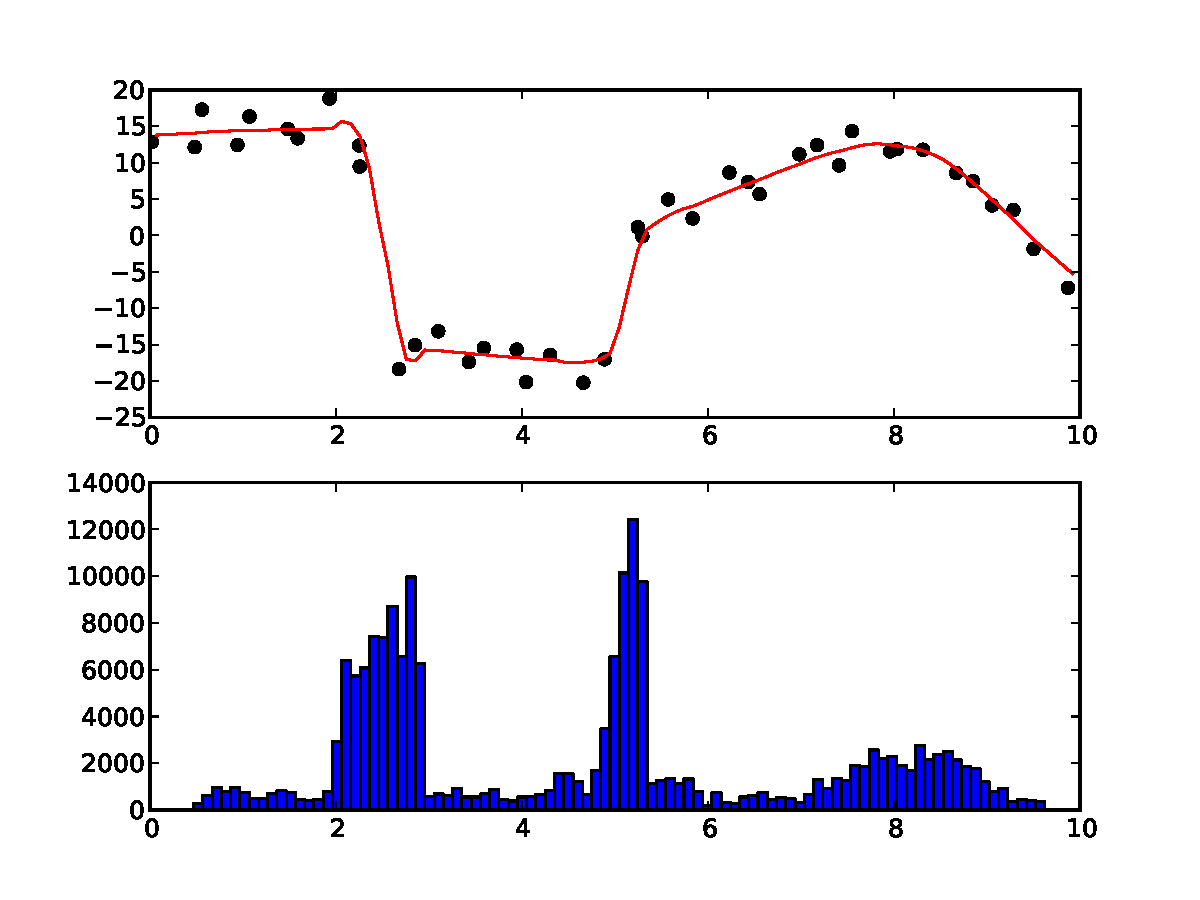
\includegraphics[width=\linewidth]{../ch2-analyse.pdf}
\caption{The Default Analysis Plot}
\label{fig:defaultanalysis}
\end{marginfigure}

In the plot, rather than just plotting the mean of the fits, we have
also plotted the histogram of the location of the partition boundaries
which indicates the most likely location of the discontinuities. As
can be seen in the figure, the histogram highlights the artificial
discontinuities created at x = 2.5 and 5.

We have also plotted the histogram of the number of partitions as 
shown in Figure~\ref{fig:defaultanalysispartcount}. From this we 
can infer the likelihood of the number of the partitions in the
data.

\begin{marginfigure}
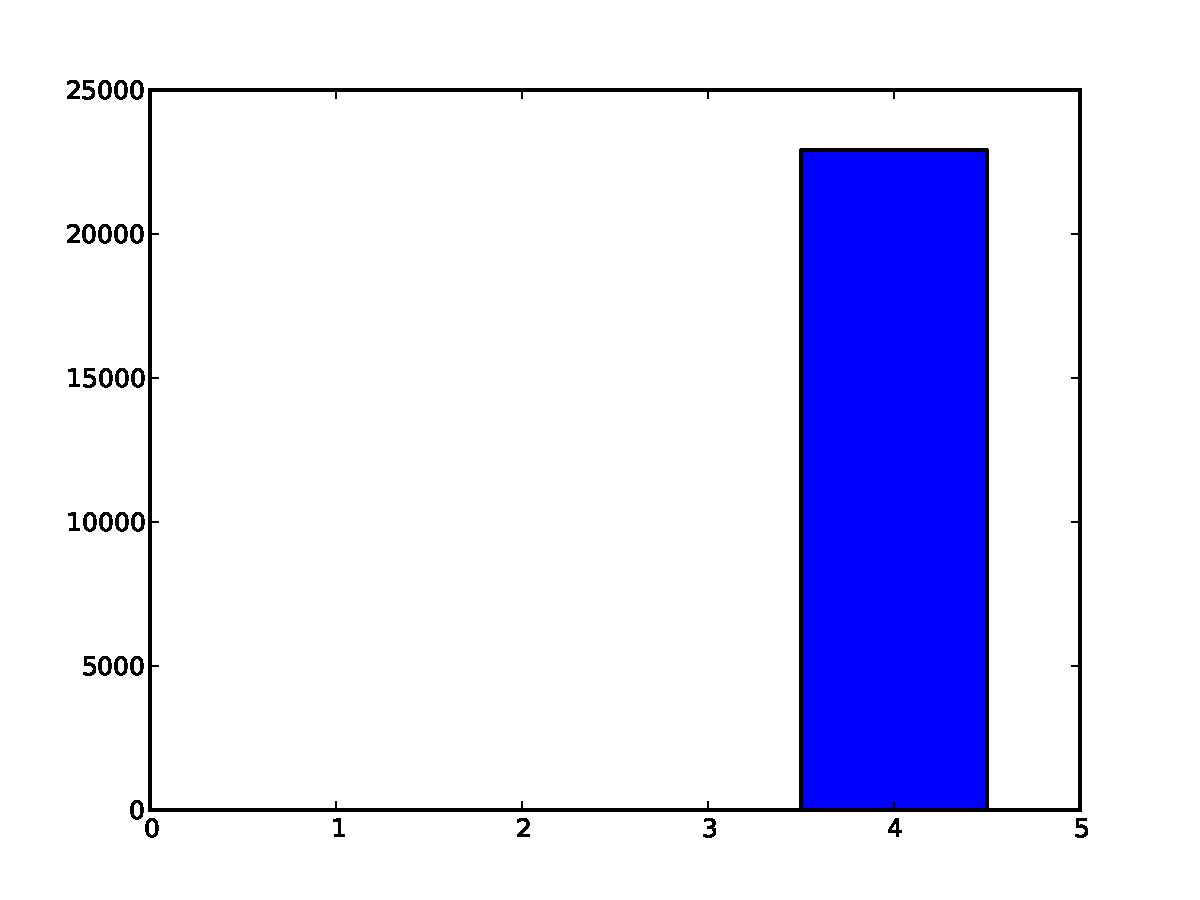
\includegraphics[width=\linewidth]{../ch2-analyse-partcount.pdf}
\caption{The Partition Count Histogram}
\label{fig:defaultanalysispartcount}
\end{marginfigure}

It should be noted here that there are two discontinuities in function and one less prominent
change in gradient in the real data. Looking at the plot of the number of partitions, we see strong support for 4 partitions,
as the algorithm has identified the four segments in the original curve.

\section{Increasing the maximum order of the polynomial}

Partition modelling and allowing higher order polynomials are in
conflict to some degree. A higher order polynomial can fit a 
discontinuity to some degree and therefore obviate the need to 
create an extra partition. 

To show this, we can increase the maximum order allowed for the 
polynomials in each partition to 5.
This means that the fitting procedure may use up to a 5th order polynomial instead
of line segments. The script to do this is shown in Listing~\ref{5th:orderanalysis}.

\lstset{caption=Increasing the maximum order of the polynomials,label=5th:orderanalysis}
\lstinputlisting{../ch3-orderanalysis.py}

The results of running this script can be seen in
Figures~\ref{fig:orderanalysis} and \ref{fig:orderanalysispartcount}.
As can be seen, the fit is more smooth than the previous analysis and
 supports a fewer number of partitions. In particular we can see that there
is some support for no discontinuities, but it is more likely that
there are 1 or 2 which matches our artificially created boundaries
(the discontinuity at x = 5 is not that large so it can be
accommodated by a higher order polynomial). Try changing the
maximum allowed order to, say, 2, i.e. allow up to a quadratic, and examine
what happens to the Partition Count Histogram.

\begin{marginfigure}
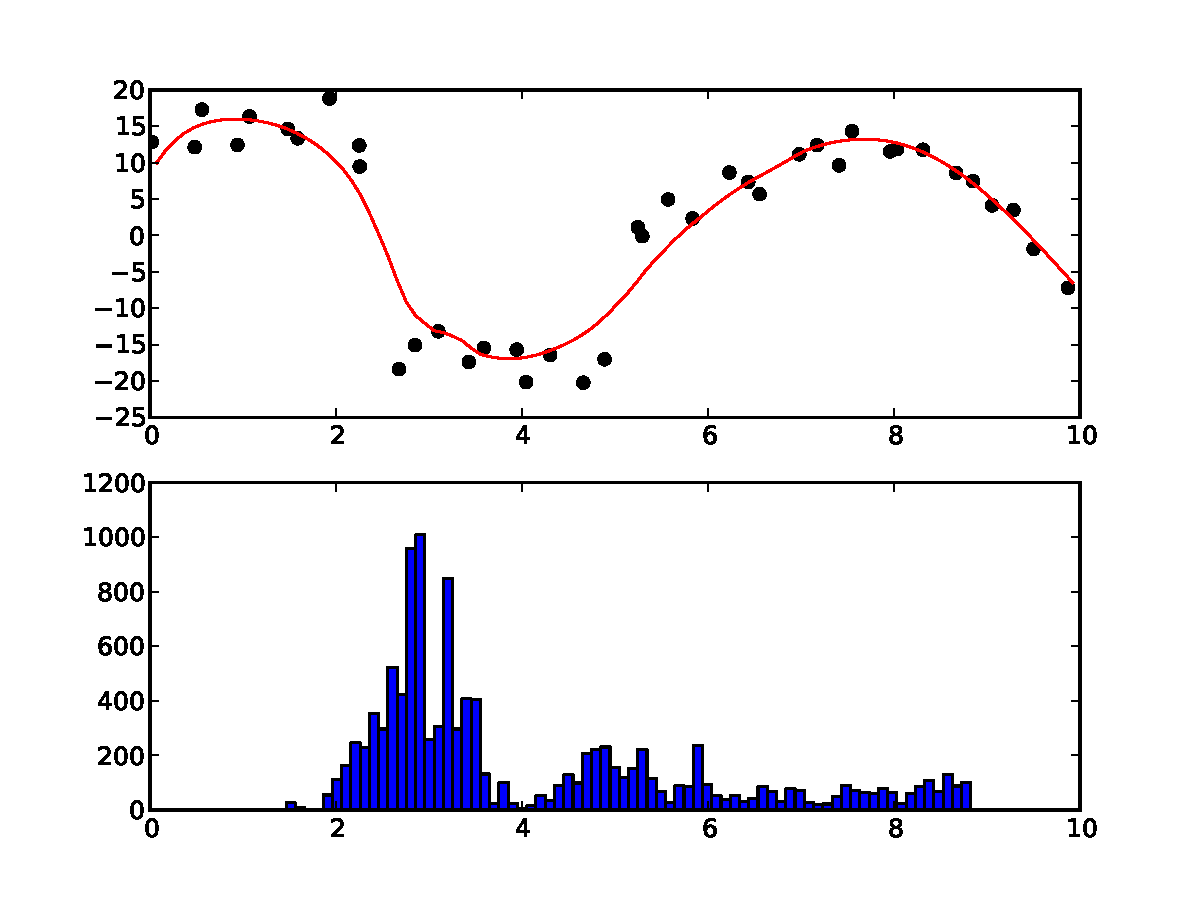
\includegraphics[width=\linewidth]{../ch3-order.pdf}
\caption{The Order Analysis Plot}
\label{fig:orderanalysis}
\end{marginfigure}


\begin{marginfigure}
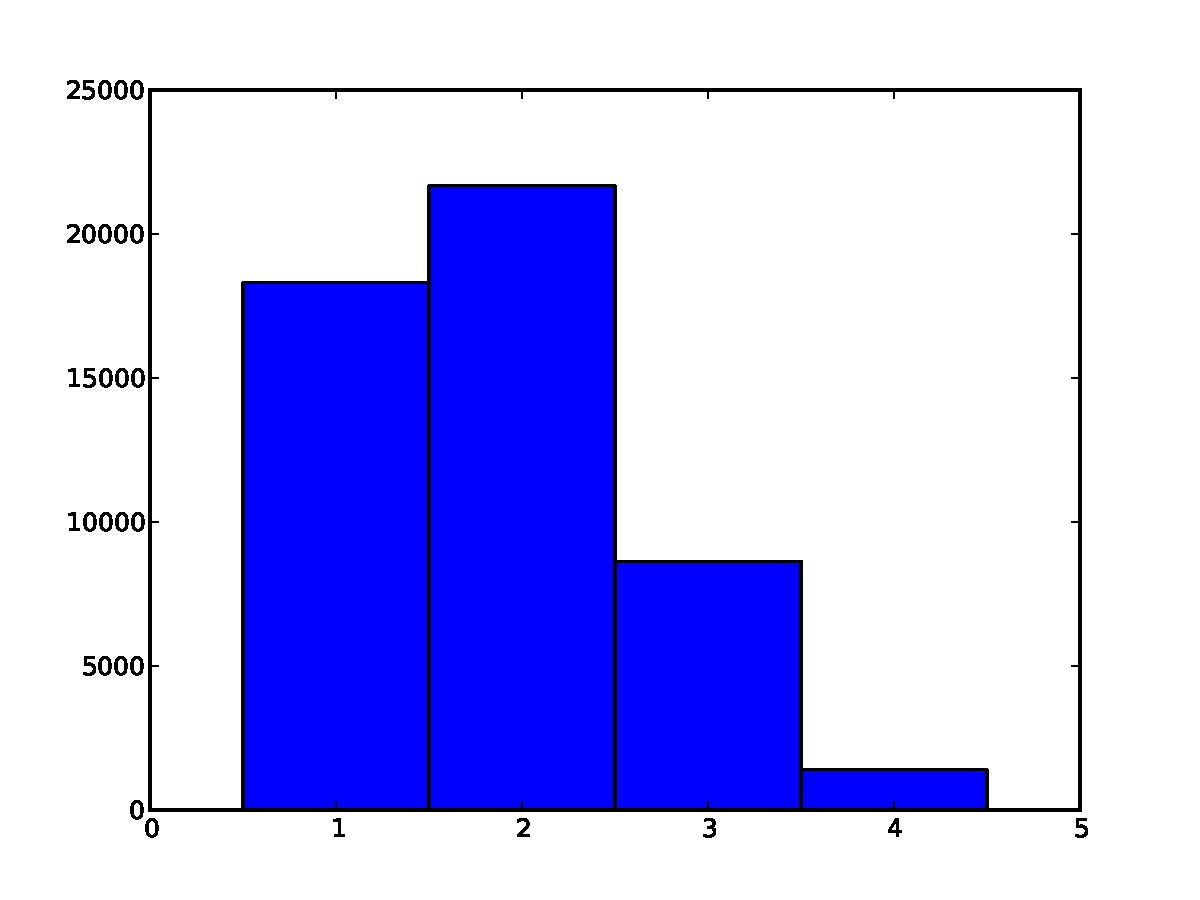
\includegraphics[width=\linewidth]{../ch3-orderpartcount.pdf}
\caption{The Partition Count Histogram}
\label{fig:orderanalysispartcount}
\end{marginfigure}

\section{Confidence}

So far we have only plotted the mean of the fits, however this gives only a glimpse
as to how the data is being fitted. One way to look at the fitting is to takes samples
of the fitting curves. The script to do this is showing in Listing~\ref{lst:confidence}.

\lstset{caption=Sampling the Fitting, label=lst:confidence}
\lstinputlisting{../ch4-confidence.py}

The resulting plot is shown in Figure~\ref{fig:confidence}. This plot shows the mean as
well as 200 curves sampled from the fitting process overplotted with transparency so that 
the darker regions are where the true curve is more likely to be. What should be noted
is that there are large spikes about the discontinuities and this is to be expected
as the fitting process will trial fitting curves across these discontinuities which 
will produce high order curves which will overshoot. 

\begin{marginfigure}
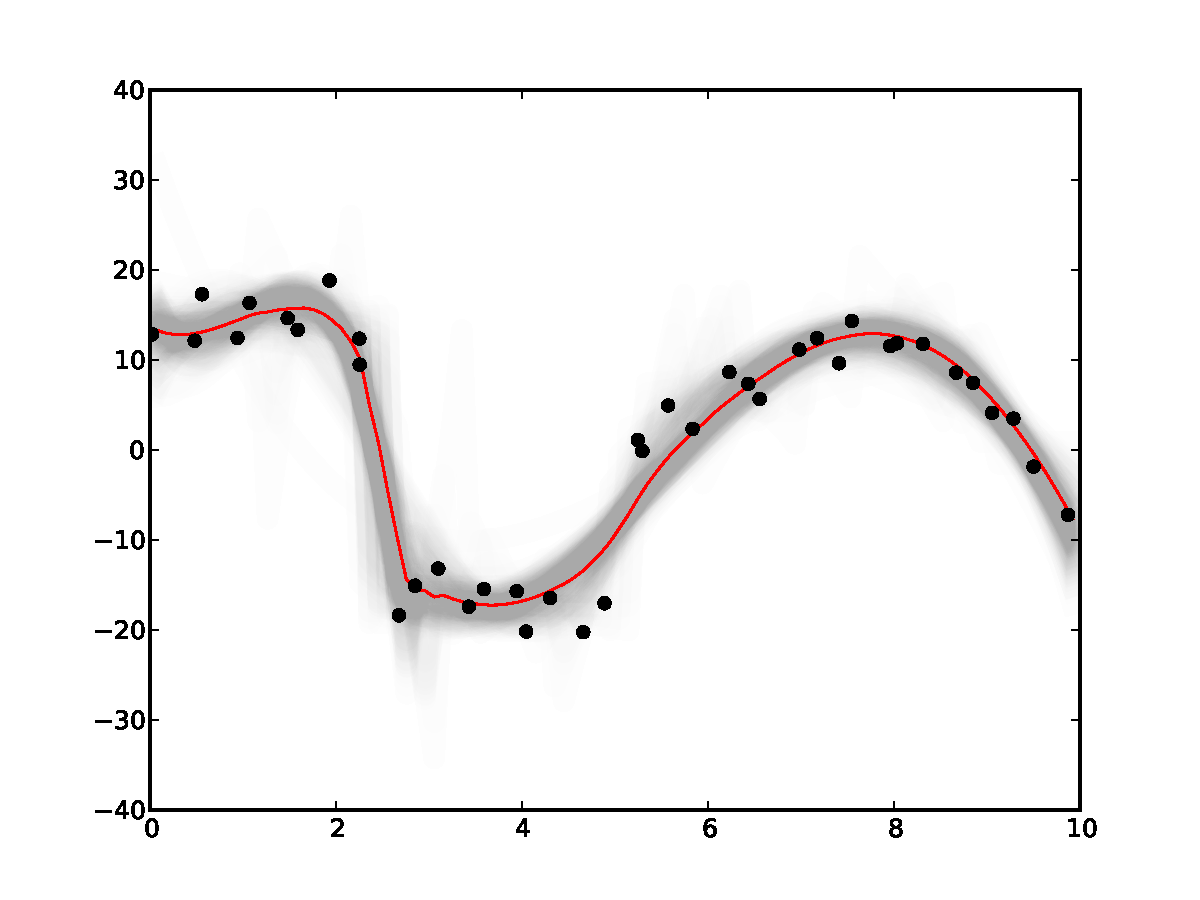
\includegraphics[width=\linewidth]{../ch4-confidence.pdf}
\caption{Sampled Curves from the Fitting}
\label{fig:confidence}
\end{marginfigure}

Another feature to notices is that at approximately x = 4.5, the
curves tends to take 2 alternate paths. This type of feature is likely
due to whether a partition boundary is located at approximately x = 5
or not.

An alternative look at the breadth of curves is to plot the confidence
intervals that are generated during the fitting process. This result
is shown in Figure~\ref{fig:confidenceintervals}.

\begin{marginfigure}
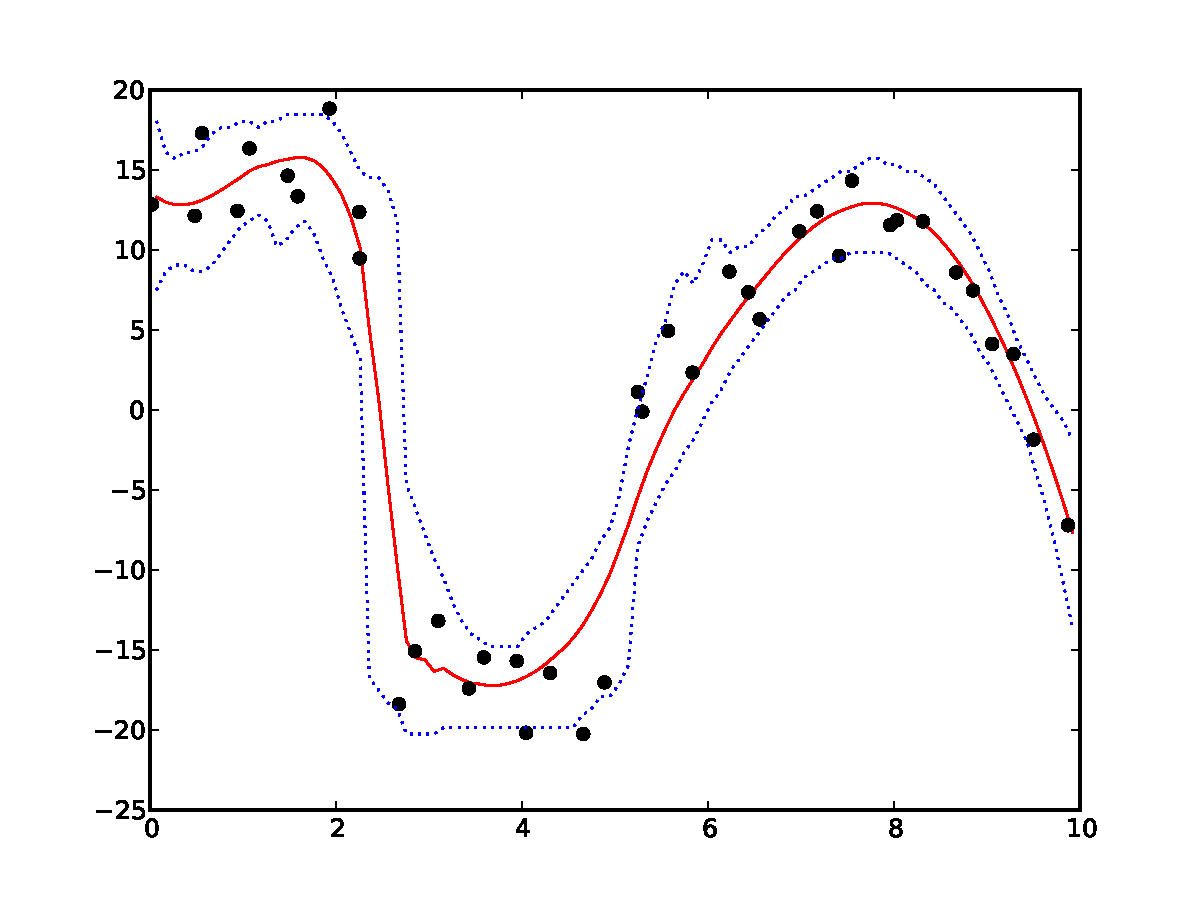
\includegraphics[width=\linewidth]{../ch4-confidenceintervals.pdf}
\caption{Confidence Intervals from the Curve Fitting}
\label{fig:confidenceintervals}
\end{marginfigure}

The confidence interval curves are shown in blue dashed lines. What
these curves represent is 95 percent of the curves generated during
the fitting process were contained within these lines. Similarly to
the sampled curves, there is some overshoot near severe
discontinuities.  Lowering the maximum order can sometimes alleviate
these.

\end{document}

